
%% bare_jrnl.tex
%% V1.3
%% 2007/01/11
%% by Michael Shell
%% see http://www.michaelshell.org/
%% for current contact information.
%%
%% This is a skeleton file demonstrating the use of IEEEtran.cls
%% (requires IEEEtran.cls version 1.7 or later) with an IEEE journal paper.
%%
%% Support sites:
%% http://www.michaelshell.org/tex/ieeetran/
%% http://www.ctan.org/tex-archive/macros/latex/contrib/IEEEtran/
%% and
%% http://www.ieee.org/



% *** Authors should verify (and, if needed, correct) their LaTeX system  ***
% *** with the testflow diagnostic prior to trusting their LaTeX platform ***
% *** with production work. IEEE's font choices can trigger bugs that do  ***
% *** not appear when using other class files.                            ***
% The testflow support page is at:
% http://www.michaelshell.org/tex/testflow/


%%*************************************************************************
%% Legal Notice:
%% This code is offered as-is without any warranty either expressed or
%% implied; without even the implied warranty of MERCHANTABILITY or
%% FITNESS FOR A PARTICULAR PURPOSE! 
%% User assumes all risk.
%% In no event shall IEEE or any contributor to this code be liable for
%% any damages or losses, including, but not limited to, incidental,
%% consequential, or any other damages, resulting from the use or misuse
%% of any information contained here.
%%
%% All comments are the opinions of their respective authors and are not
%% necessarily endorsed by the IEEE.
%%
%% This work is distributed under the LaTeX Project Public License (LPPL)
%% ( http://www.latex-project.org/ ) version 1.3, and may be freely used,
%% distributed and modified. A copy of the LPPL, version 1.3, is included
%% in the base LaTeX documentation of all distributions of LaTeX released
%% 2003/12/01 or later.
%% Retain all contribution notices and credits.
%% ** Modified files should be clearly indicated as such, including  **
%% ** renaming them and changing author support contact information. **
%%
%% File list of work: IEEEtran.cls, IEEEtran_HOWTO.pdf, bare_adv.tex,
%%                    bare_conf.tex, bare_jrnl.tex, bare_jrnl_compsoc.tex
%%*************************************************************************

% Note that the a4paper option is mainly intended so that authors in
% countries using A4 can easily print to A4 and see how their papers will
% look in print - the typesetting of the document will not typically be
% affected with changes in paper size (but the bottom and side margins will).
% Use the testflow package mentioned above to verify correct handling of
% both paper sizes by the user's LaTeX system.
%
% Also note that the "draftcls" or "draftclsnofoot", not "draft", option
% should be used if it is desired that the figures are to be displayed in
% draft mode.
%
\documentclass[draftclsnofoot,12pt,journal,onecolumn]{IEEEtran}
\renewcommand{\rmdefault}{phv} % Arial
\renewcommand{\sfdefault}{phv} % Arial
\setcounter{page}{3}

%
% If IEEEtran.cls has not been installed into the LaTeX system files,
% manually specify the path to it like:
% \documentclass[journal]{../sty/IEEEtran}





% Some very useful LaTeX packages include:
% (uncomment the ones you want to load)


% *** MISC UTILITY PACKAGES ***
%
%\usepackage{ifpdf}
% Heiko Oberdiek's ifpdf.sty is very useful if you need conditional
% compilation based on whether the output is pdf or dvi.
% usage:
% \ifpdf
%   % pdf code
% \else
%   % dvi code
% \fi
% The latest version of ifpdf.sty can be obtained from:
% http://www.ctan.org/tex-archive/macros/latex/contrib/oberdiek/
% Also, note that IEEEtran.cls V1.7 and later provides a builtin
% \ifCLASSINFOpdf conditional that works the same way.
% When switching from latex to pdflatex and vice-versa, the compiler may
% have to be run twice to clear warning/error messages.






% *** CITATION PACKAGES ***
%
\usepackage{cite}
% cite.sty was written by Donald Arseneau
% V1.6 and later of IEEEtran pre-defines the format of the cite.sty package
% \cite{} output to follow that of IEEE. Loading the cite package will
% result in citation numbers being automatically sorted and properly
% "compressed/ranged". e.g., [1], [9], [2], [7], [5], [6] without using
% cite.sty will become [1], [2], [5]--[7], [9] using cite.sty. cite.sty's
% \cite will automatically add leading space, if needed. Use cite.sty's
% noadjust option (cite.sty V3.8 and later) if you want to turn this off.
% cite.sty is already installed on most LaTeX systems. Be sure and use
% version 4.0 (2003-05-27) and later if using hyperref.sty. cite.sty does
% not currently provide for hyperlinked citations.
% The latest version can be obtained at:
% http://www.ctan.org/tex-archive/macros/latex/contrib/cite/
% The documentation is contained in the cite.sty file itself.



%\usepackage{hyperref}


% *** GRAPHICS RELATED PACKAGES ***
%
\ifCLASSINFOpdf
  % \usepackage[pdftex]{graphicx}
  % declare the path(s) where your graphic files are
  % \graphicspath{{../pdf/}{../jpeg/}}
  % and their extensions so you won't have to specify these with
  % every instance of \includegraphics
  % \DeclareGraphicsExtensions{.pdf,.jpeg,.png}
\else
  % or other class option (dvipsone, dvipdf, if not using dvips). graphicx
  % will default to the driver specified in the system graphics.cfg if no
  % driver is specified.
   \usepackage[dvips]{graphicx}
  % declare the path(s) where your graphic files are
  \graphicspath{{./figures/}}
  % and their extensions so you won't have to specify these with
  % every instance of \includegraphics
   \DeclareGraphicsExtensions{.eps}
\fi
% graphicx was written by David Carlisle and Sebastian Rahtz. It is
% required if you want graphics, photos, etc. graphicx.sty is already
% installed on most LaTeX systems. The latest version and documentation can
% be obtained at: 
% http://www.ctan.org/tex-archive/macros/latex/required/graphics/
% Another good source of documentation is "Using Imported Graphics in
% LaTeX2e" by Keith Reckdahl which can be found as epslatex.ps or
% epslatex.pdf at: http://www.ctan.org/tex-archive/info/
%
% latex, and pdflatex in dvi mode, support graphics in encapsulated
% postscript (.eps) format. pdflatex in pdf mode supports graphics
% in .pdf, .jpeg, .png and .mps (metapost) formats. Users should ensure
% that all non-photo figures use a vector format (.eps, .pdf, .mps) and
% not a bitmapped formats (.jpeg, .png). IEEE frowns on bitmapped formats
% which can result in "jaggedy"/blurry rendering of lines and letters as
% well as large increases in file sizes.
%
% You can find documentation about the pdfTeX application at:
% http://www.tug.org/applications/pdftex





% *** MATH PACKAGES ***
%
\usepackage[cmex10]{amsmath}
\usepackage{amsfonts}
% A popular package from the American Mathematical Society that provides
% many useful and powerful commands for dealing with mathematics. If using
% it, be sure to load this package with the cmex10 option to ensure that
% only type 1 fonts will utilized at all point sizes. Without this option,
% it is possible that some math symbols, particularly those within
% footnotes, will be rendered in bitmap form which will result in a
% document that can not be IEEE Xplore compliant!
%
% Also, note that the amsmath package sets \interdisplaylinepenalty to 10000
% thus preventing page breaks from occurring within multiline equations. Use:
%\interdisplaylinepenalty=2500
% after loading amsmath to restore such page breaks as IEEEtran.cls normally
% does. amsmath.sty is already installed on most LaTeX systems. The latest
% version and documentation can be obtained at:
% http://www.ctan.org/tex-archive/macros/latex/required/amslatex/math/





% *** SPECIALIZED LIST PACKAGES ***
%
%\usepackage{algorithmic}
% algorithmic.sty was written by Peter Williams and Rogerio Brito.
% This package provides an algorithmic environment fo describing algorithms.
% You can use the algorithmic environment in-text or within a figure
% environment to provide for a floating algorithm. Do NOT use the algorithm
% floating environment provided by algorithm.sty (by the same authors) or
% algorithm2e.sty (by Christophe Fiorio) as IEEE does not use dedicated
% algorithm float types and packages that provide these will not provide
% correct IEEE style captions. The latest version and documentation of
% algorithmic.sty can be obtained at:
% http://www.ctan.org/tex-archive/macros/latex/contrib/algorithms/
% There is also a support site at:
% http://algorithms.berlios.de/index.html
% Also of interest may be the (relatively newer and more customizable)
% algorithmicx.sty package by Szasz Janos:
% http://www.ctan.org/tex-archive/macros/latex/contrib/algorithmicx/




% *** ALIGNMENT PACKAGES ***
%
%\usepackage{array}
% Frank Mittelbach's and David Carlisle's array.sty patches and improves
% the standard LaTeX2e array and tabular environments to provide better
% appearance and additional user controls. As the default LaTeX2e table
% generation code is lacking to the point of almost being broken with
% respect to the quality of the end results, all users are strongly
% advised to use an enhanced (at the very least that provided by array.sty)
% set of table tools. array.sty is already installed on most systems. The
% latest version and documentation can be obtained at:
% http://www.ctan.org/tex-archive/macros/latex/required/tools/


%\usepackage{mdwmath}
%\usepackage{mdwtab}
% Also highly recommended is Mark Wooding's extremely powerful MDW tools,
% especially mdwmath.sty and mdwtab.sty which are used to format equations
% and tables, respectively. The MDWtools set is already installed on most
% LaTeX systems. The lastest version and documentation is available at:
% http://www.ctan.org/tex-archive/macros/latex/contrib/mdwtools/


% IEEEtran contains the IEEEeqnarray family of commands that can be used to
% generate multiline equations as well as matrices, tables, etc., of high
% quality.


%\usepackage{eqparbox}
% Also of notable interest is Scott Pakin's eqparbox package for creating
% (automatically sized) equal width boxes - aka "natural width parboxes".
% Available at:
% http://www.ctan.org/tex-archive/macros/latex/contrib/eqparbox/





% *** SUBFIGURE PACKAGES ***
\usepackage[tight,footnotesize]{subfigure}
% subfigure.sty was written by Steven Douglas Cochran. This package makes it
% easy to put subfigures in your figures. e.g., "Figure 1a and 1b". For IEEE
% work, it is a good idea to load it with the tight package option to reduce
% the amount of white space around the subfigures. subfigure.sty is already
% installed on most LaTeX systems. The latest version and documentation can
% be obtained at:
% http://www.ctan.org/tex-archive/obsolete/macros/latex/contrib/subfigure/
% subfigure.sty has been superceeded by subfig.sty.



%\usepackage[caption=false]{caption}
%\usepackage[font=footnotesize,caption=false]{subfig}
% subfig.sty, also written by Steven Douglas Cochran, is the modern
% replacement for subfigure.sty. However, subfig.sty requires and
% automatically loads Axel Sommerfeldt's caption.sty which will override
% IEEEtran.cls handling of captions and this will result in nonIEEE style
% figure/table captions. To prevent this problem, be sure and preload
% caption.sty with its "caption=false" package option. This is will preserve
% IEEEtran.cls handing of captions. Version 1.3 (2005/06/28) and later 
% (recommended due to many improvements over 1.2) of subfig.sty supports
% the caption=false option directly:
%\usepackage[caption=false,font=footnotesize]{subfig}
%
% The latest version and documentation can be obtained at:
% http://www.ctan.org/tex-archive/macros/latex/contrib/subfig/
% The latest version and documentation of caption.sty can be obtained at:
% http://www.ctan.org/tex-archive/macros/latex/contrib/caption/




% *** FLOAT PACKAGES ***
%
%\usepackage{fixltx2e}
% fixltx2e, the successor to the earlier fix2col.sty, was written by
% Frank Mittelbach and David Carlisle. This package corrects a few problems
% in the LaTeX2e kernel, the most notable of which is that in current
% LaTeX2e releases, the ordering of single and double column floats is not
% guaranteed to be preserved. Thus, an unpatched LaTeX2e can allow a
% single column figure to be placed prior to an earlier double column
% figure. The latest version and documentation can be found at:
% http://www.ctan.org/tex-archive/macros/latex/base/



%\usepackage{stfloats}
% stfloats.sty was written by Sigitas Tolusis. This package gives LaTeX2e
% the ability to do double column floats at the bottom of the page as well
% as the top. (e.g., "\begin{figure*}[!b]" is not normally possible in
% LaTeX2e). It also provides a command:
%\fnbelowfloat
% to enable the placement of footnotes below bottom floats (the standard
% LaTeX2e kernel puts them above bottom floats). This is an invasive package
% which rewrites many portions of the LaTeX2e float routines. It may not work
% with other packages that modify the LaTeX2e float routines. The latest
% version and documentation can be obtained at:
% http://www.ctan.org/tex-archive/macros/latex/contrib/sttools/
% Documentation is contained in the stfloats.sty comments as well as in the
% presfull.pdf file. Do not use the stfloats baselinefloat ability as IEEE
% does not allow \baselineskip to stretch. Authors submitting work to the
% IEEE should note that IEEE rarely uses double column equations and
% that authors should try to avoid such use. Do not be tempted to use the
% cuted.sty or midfloat.sty packages (also by Sigitas Tolusis) as IEEE does
% not format its papers in such ways.


%\ifCLASSOPTIONcaptionsoff
%  \usepackage[nomarkers]{endfloat}
% \let\MYoriglatexcaption\caption
% \renewcommand{\caption}[2][\relax]{\MYoriglatexcaption[#2]{#2}}
%\fi
% endfloat.sty was written by James Darrell McCauley and Jeff Goldberg.
% This package may be useful when used in conjunction with IEEEtran.cls'
% captionsoff option. Some IEEE journals/societies require that submissions
% have lists of figures/tables at the end of the paper and that
% figures/tables without any captions are placed on a page by themselves at
% the end of the document. If needed, the draftcls IEEEtran class option or
% \CLASSINPUTbaselinestretch interface can be used to increase the line
% spacing as well. Be sure and use the nomarkers option of endfloat to
% prevent endfloat from "marking" where the figures would have been placed
% in the text. The two hack lines of code above are a slight modification of
% that suggested by in the endfloat docs (section 8.3.1) to ensure that
% the full captions always appear in the list of figures/tables - even if
% the user used the short optional argument of \caption[]{}.
% IEEE papers do not typically make use of \caption[]'s optional argument,
% so this should not be an issue. A similar trick can be used to disable
% captions of packages such as subfig.sty that lack options to turn off
% the subcaptions:
% For subfig.sty:
% \let\MYorigsubfloat\subfloat
% \renewcommand{\subfloat}[2][\relax]{\MYorigsubfloat[]{#2}}
% For subfigure.sty:
% \let\MYorigsubfigure\subfigure
% \renewcommand{\subfigure}[2][\relax]{\MYorigsubfigure[]{#2}}
% However, the above trick will not work if both optional arguments of
% the \subfloat/subfig command are used. Furthermore, there needs to be a
% description of each subfigure *somewhere* and endfloat does not add
% subfigure captions to its list of figures. Thus, the best approach is to
% avoid the use of subfigure captions (many IEEE journals avoid them anyway)
% and instead reference/explain all the subfigures within the main caption.
% The latest version of endfloat.sty and its documentation can obtained at:
% http://www.ctan.org/tex-archive/macros/latex/contrib/endfloat/
%
% The IEEEtran \ifCLASSOPTIONcaptionsoff conditional can also be used
% later in the document, say, to conditionally put the References on a 
% page by themselves.





% *** PDF, URL AND HYPERLINK PACKAGES ***
%
\usepackage{url}
% url.sty was written by Donald Arseneau. It provides better support for
% handling and breaking URLs. url.sty is already installed on most LaTeX
% systems. The latest version can be obtained at:
% http://www.ctan.org/tex-archive/macros/latex/contrib/misc/
% Read the url.sty source comments for usage information. Basically,
% \url{my_url_here}.

\usepackage{pgfgantt}


\usepackage{fancyhdr}
\usepackage{lastpage}
\renewcommand{\headheight}{0.4in}
\setlength{\headwidth}{\textwidth}
\fancyhead[L]{
  
\includegraphics[height=0.15in]{COM4EU_Logo}
}
\fancyhead[R]{ % right
C4EU 5.5.2: Report on support actions - Training and Networking -b
}
\pagestyle{fancy}
\cfoot{Page \thepage\ of \pageref{LastPage}}



% *** Do not adjust lengths that control margins, column widths, etc. ***
% *** Do not use packages that alter fonts (such as pslatex).         ***
% There should be no need to do such things with IEEEtran.cls V1.6 and later.
% (Unless specifically asked to do so by the journal or conference you plan
% to submit to, of course. )


% correct bad hyphenation here
\hyphenation{op-tical net-works semi-conduc-tor}


\begin{document}
%
% paper title
% can use linebreaks \\ within to get better formatting as desired
\title{Building a BuB Community \\ (C4EU 5.5.2: Report on support actions - training and networking -b )}
%
%
% author names and IEEE memberships
% note positions of commas and nonbreaking spaces ( ~ ) LaTeX will not break
% a structure at a ~ so this keeps an author's name from being broken across
% two lines.
% use \thanks{} to gain access to the first footnote area
% a separate \thanks must be used for each paragraph as LaTeX2e's \thanks
% was not built to handle multiple paragraphs
%

\author{
	Name~Surname, %\IEEEmembership{Member,~IEEE,}
	Name~Surname, %\IEEEmembership{Member,~IEEE,}
	Name~Surname, %\IEEEmembership{Member,~IEEE,}
	Name~Surname, %\IEEEmembership{Member,~IEEE,}
	Name~Surname, %\IEEEmembership{Member,~IEEE,}
    and~Name~Surname% \IEEEmembership{Life~Fellow,~IEEE}% <-this % stops a space
\thanks{
The authors are with Universitat Pompeu Fabra
}
}


% note the % following the last \IEEEmembership and also \thanks - 
% these prevent an unwanted space from occurring between the last author name
% and the end of the author line. i.e., if you had this:
% 
% \author{....lastname \thanks{...} \thanks{...} }
%                     ^------------^------------^----Do not want these spaces!
%
% a space would be appended to the last name and could cause every name on that
% line to be shifted left slightly. This is one of those "LaTeX things". For
% instance, "\textbf{A} \textbf{B}" will typeset as "A B" not "AB". To get
% "AB" then you have to do: "\textbf{A}\textbf{B}"
% \thanks is no different in this regard, so shield the last } of each \thanks
% that ends a line with a % and do not let a space in before the next \thanks.
% Spaces after \IEEEmembership other than the last one are OK (and needed) as
% you are supposed to have spaces between the names. For what it is worth,
% this is a minor point as most people would not even notice if the said evil
% space somehow managed to creep in.



% The paper headers
\markboth{C4EU 5.5.2: Report on support actions - Training and Networking - b}%
{C4EU 5.5.2: Report on support actions - Training and Networking -b}
% The only time the second header will appear is for the odd numbered pages
% after the title page when using the twoside option.
% 
% *** Note that you probably will NOT want to include the author's ***
% *** name in the headers of peer review papers.                   ***
% You can use \ifCLASSOPTIONpeerreview for conditional compilation here if
% you desire.




% If you want to put a publisher's ID mark on the page you can do it like
% this:
%\IEEEpubid{0000--0000/00\$00.00~\copyright~2007 IEEE}
% Remember, if you use this you must call \IEEEpubidadjcol in the second
% column for its text to clear the IEEEpubid mark.



% use for special paper notices
%\IEEEspecialpapernotice{(Invited Paper)}




% make the title area
\maketitle
\thispagestyle{fancy}

\begin{abstract}
%\boldmath
This report summarizes the training, networking and communication efforts of the BuB4EU branch of the Commons for Europe project.
At the time of this writing, the fellows recruited for the second round of botto-up broadband pilots are already working.
Each of the fellows has both one academic advisor and one mentor with extensive BuB experience.
These two roles complement each other in the education of the student.
The collaboration tools are those commonly present in collaborative initiatives: workshops, mailing list, and a git repository.
We complement the training of the fellows with the training of the general public using an online course.
The goal of this course is to empower the citizens to be able to reproduce one of the pilots that was executed in the first round: the open wireless sensor network.
\end{abstract}
% IEEEtran.cls defaults to using nonbold math in the Abstract.
% This preserves the distinction between vectors and scalars. However,
% if the journal you are submitting to favors bold math in the abstract,
% then you can use LaTeX's standard command \boldmath at the very start
% of the abstract to achieve this. Many IEEE journals frown on math
% in the abstract anyway.

% Note that keywords are not normally used for peerreview papers.
\begin{IEEEkeywords}
 Bottom-up-Broadband (BuB), training, workshops, presentations
%Slotted Aloha, game theory, contention control, media access control.
\end{IEEEkeywords}

\clearpage

\tableofcontents

\clearpage

\listoffigures

\listoftables

\clearpage




% For peer review papers, you can put extra information on the cover
% page as needed:
% \ifCLASSOPTIONpeerreview
% \begin{center} \bfseries EDICS Category: 3-BBND \end{center}
% \fi
%
% For peerreview papers, this IEEEtran command inserts a page break and
% creates the second title. It will be ignored for other modes.
\IEEEpeerreviewmaketitle



\section{Introduction}
% The very first letter is a 2 line initial drop letter followed
% by the rest of the first word in caps.
% 
% form to use if the first word consists of a single letter:
% \IEEEPARstart{A}{demo} file is ....
% 
% form to use if you need the single drop letter followed by
% normal text (unknown if ever used by IEEE):
% \IEEEPARstart{A}{}demo file is ....
% 
% Some journals put the first two words in caps:
% \IEEEPARstart{T}{his demo} file is ....
% 
% Here we have the typical use of a "T" for an initial drop letter
% and "HIS" in caps to complete the first word.
\IEEEPARstart{T}{his} report summarizes the training and communication efforts of the BuB4EU branch of the Commons for Europe project.
After this introduction, Section \ref{sec:about} provides information about this document and how to collaborate.
Section \ref{sec:fellows} introduces the fellow program that we have prepared to back the execution of the selected pilots.
Section \ref{sec:mentor} describes the roles of mentor and adacemic advisor that will help the fellows participating in the pilots.
Those that are interested in BuB4EU meet in the workshops detailed in Section \ref{sec:workshops} and participate in the mailing list as explained in Section \ref{sec:mailing}.
A web has been constructed and is continually evolving as explained in \ref{sec:web}.
The BuB4EU branch and the obtained results have also been presented bottom-up broadband forums that are introduced in Section \ref{sec:forums}.
The plan for the preparation of an online course is detailed in~\ref{sec:online}.
Finally, Section \ref{sec:conclusion} offers some concluding remarks.

\section{About this document}
\label{sec:about}

This report has been produced using open source tools such as {\LaTeX} \cite{lamport1994ldp} and \emph{git} \cite{chacon2009pg}.
{\LaTeX} is widely used in academia to prepare print-class documents.
It automatically takes care of numbering, cross-referencing, tables of contents, bibliography, etc.
\emph{Git} is a high performance distributed revision control which is used in many open source projects, such as the linux kernel.
Git makes it easy and safe to collaborate as each contributor works on his own personal copy.
Good contributions can be easily shared with others, and it is always possible to revert to a previous version.

Our git repository is publicly available in \emph{github}:

https://github.com/jbarcelo/C4EU-deliverables

Anyone who is familiar with {\LaTeX} and \emph{github} can contribute to this document.
The firs step is to make a copy (a \emph{fork} in \emph{github} jargon).
The contributor can work in this copy and make changes to improve the document.
After that, it is necessary to request that these changes are merged into the original copy of the document (a \emph{pull request} in github jargon).

If you see anything that can be improved, feel free to contribute.
This document is alive in the sense that it will keep evolving as long as contributors make changes and improve it.

The system automatically keeps track of all the contributors and their contributions.
It is possible to see who is contributing more actively and which are the exact changes made by each contributor.
And everything is public on the web.

\section{Fellow program for supporting BuB pilots}
\label{sec:fellows}

Each of the pilots selected for execution receives the backing of a fellow.
Fellows are recruited among the last year students of a four year networking undergraduate program.
The selection process relies on academic grades, Curriculum Vitae and personal interview.

For project management purposes, each fellow has to prepare four different deliverables regarding the pilot.
First, a pilot charter which is a high-level description of the pilot.
Then, a detailed planning with the tasks to be carried out throughout the pilot execution.
When the first results are available, they will be covered by an execution deliverable.
This execution deliverable is a checkpoint to verify that the pilot is on track and advancing according the schedule.
Finally, upon completion of the pilot, the fellow will prepare a memory for publication and will explain the pilot in a public presentation.

The Bottom-up Broadband fellows will participate in a join training 3-days session with the Code for Europe fellows organized by the project co-ordinator ESADE.
Besides this sessions, they are receiving intensive training and support combining the different tools described in the remainder of this document.

\section{Mentor program and academic advice}
\label{sec:mentor}
The fellows selected to participate in the Commons for Europe (C4EU) project do so as part of their education at the university.
Specifically, this training is divided in two different blocks: \emph{practicum} and \emph{degree thesis}.
The practicum involves real-world work in which the fellows have the opportunity to use the skills they have learned in regular courses.
It is also the opportunity to realize that real-world work is far away from the courses taught at the university, which means that the fellows have to make an extra effort to get acquainted with technologies and work-flows that they have not learned in class.

The \emph{practicum} is not a controlled environment as the course lab assignments are.
Things can go wrong, and it is important to understand and accept it.
Furthermore, there is not a teacher that \emph{knows the solution}.
This means that the level of effort to achieve results is much higher in the practicum than in a course assignment, as it is possible to get stuck and it may take days or longer to find a solution or a workaround.
The effort is measured in the European Credit Transfer System (ECTS).
The \emph{practicum} has a value of 20 ECTS credits, which is equivalent to 500 hours of work.

The fellows are not alone in this quest.
A \emph{mentor} is assigned to each student to indicate the tasks that the student has to do and provide the necessary help and guidance.
As the practicum is tied to a real-world work, the \emph{mentor} needs to be someone that has been working in this real-world for some time.

Besides the actual technical skills acquired in the execution of the \emph{practicum}, the fellows are also expected to practice \emph{soft} skills such as participation in meetings, effective communication, organization of work to meet schedules, generation of documentation, etc.
For some people, the practicum can be the starting point of a professional career.

A mentor has been assigned to each of the student participating in the C4EU project.
It is important that the mentor is someone from outside the university that is very familiar with bottom-up-broadband and with the pilot.
Table \ref{tab:mentors} summarizes the pilots under consideration, the student assigned to each pilot and the mentor assigned to each student.

\begin{table}[!t]
%% increase table row spacing, adjust to taste
\renewcommand{\arraystretch}{1.3}
% if using array.sty, it might be a good idea to tweak the value of
%\extrarowheight as needed to properly center the text within the cells
\caption{Pilots, fellows and mentors}
\label{tab:mentors}
\centering
\begin{tabular}{|c|c|c|c|}
\hline
Pilot & Student & Mentor & Main Academic Advisor\\
\hline
Open Sensor Network & Alejandro Andreu & Alex Posada and Tomas Diez & Jaume Barcelo\\
Free Europe WiFi & Ignacio Justel & Givanni Calcerano & Albert Domingo\\
FFTx & Jorge Beltran & Roger Baig & Jaume Barcelo\\
Mobile Node & Fernando Gros & Efrain Foglia & Jaume Barcelo\\
\hline
\end{tabular}
\end{table}

In addition to the \emph{practicum}, the fellows also have write their \emph{degree thesis}.
This thesis is an academic document that is necessary to obtain the degree.
In the thesis, the fellows will comprehensively describe their pilot.
As an academic document, it has to be carefully written, well structured and profusely documented.
It is necessary to include introductory material, related work and references.
It is also important to include a detailed work-plan with descriptions of the tasks.
The work should be described in such a way that an external evaluator can understand what is the contribution and why it is important. The role of the academic advisor is to guide the fellows in the successful completion of the academic work in coordination with the mentor.

The \emph{thesis} has also a value of 20 ECTS credits, which means 500 additional hours of work.
This part of the work will be supervised by an academic advisor from the university.
There is hard deadline for the \emph{thesis} in June.
Not meeting this deadline would represent a delay of one year in the obtention of the degree.
For this reason, it may be a good idea to plan the work in such a way that the thesis is finished considerably earlier, to have some \emph{safety margin} in case of unexpected events.

\LaTeX\  is a popular document preparation system in the academia, that we will also use in the preparation of the thesis.
It is convenient to structure a large document in chapters, sections and subsection.
It also provides support for references and cross-references.
And automatically generates tables of contents, tables of figures, bibliography, etc.
Our idea is to use \LaTeX\ also for the preparation of the documentation of the C4EU project, in such a way that it can be re-used in the preparation of the thesis of the fellows.

Another tool that can be helpful in the preparation of the documentation is github.
Github is a web based extension of the git revision control system, and makes it possible that different people work in parallel on the same document, suggest changes, rollback modifications, etc. in a distributed fashion.

\subsection{Mentors for the OSN pilot}

Recently two researches joined the initiative and they will be helping the fellow to complete the pilot. A short biography is shown below.

\begin{itemize}
    \item \emph{Alex Posada}: He is an engineer who researches in the field of interactive media, produces and creates music and is actively involved in many interactive projects which normally involve sensors. Hence he will be able to contribute to the Open Sensor Network project.
    \item \emph{Tomas Diez}: He is the project manager in FabLab Barcelona ---workshop offering personal digital fabrication---, located in the Institute for Advanced Architecture of Catalonia (IAAC). He has executed projects in Latin America as well as in Europe. He focuses on the research for a more fluid language between machines and humans, and is currently working on Smart Citizen, a very similar initiative to Open Sensor Network.
\end{itemize}

\subsection{Mentor for the FFTx pilot}
The mentor for the FFTx pilot is Roger Baig Vi�as and he will help Jorge Beltran to perform this project. Roger is from Barcelona and he studied Industrial and Electronic Engineering at Universitat Polit�cnica de Catalunya (UPC). He also did a master at Universitat Aut�noma de Barcelona (UAB). 
Now he is working in the Private Foundation guifi.net by the Open, Free and Neutral Network where he does tasks as international projects, dissemination and promotion. Roger also takes part in CONFINE (FP7) and C4EU (CIP) projects.


\subsection{Mentor for the FEW pilot}
As explained before, Nacho Justel will be guided by Giovanni Calcerano from Provicia WiFi.
Giovanni is graduated in Mathematics, and developed his carrer mostly as consultant in the field of high-level technical computing / scientific / statistical experience with over ten-year experience in the business sector. He is currently working at Provincia di Roma, being the responsably of European projects as OpenData, among others.
For more information, about his professional career, you can take a look at his LinkedIn profile.

\subsection{Mentor for the Mobile Node pilot}
Fernando, will be guided by Efra\'in Foglia. Efra\'in has been working in different areas related to Design and Art. Nowadays he is doing research on the field of the relation between Design \& Art and digital networks, taking into account also their social and political implications. He is an active member of guifi.net and exo.cat, two platforms which work on the design and deployment of open networks. 
\par 
He graduated in Design of Graphic Communication in UAM (Mexico) and is currently working on his PhD at the Universitat de Barcelona (UB) about "`\textit{Art in MediaCity}"'     


\section{BuB4EU Workshops}
\label{sec:workshops}
Together with the mailing list, one of the main tools to exchange results and foster the discussion is the organization of workshops.
This workshops are announced on the mailing list and are open for everyone to participate.
There are two differentiated participation options: attendant and speaker.

The speakers are those that are more deeply involved in the project and prepare a short paper (one page) and some supporting slides for the talk.
The attendants simply listen and offer comments and feedback.

Each of the workshops has been organized by one of the members of the team.

\subsection{1st BuBEU workshop}

Date: July 24th.

Organizer: Jaume Barcelo

Attendants: 
\begin{itemize}
	\item Daniele Arena
    \item Roger Baig
	\item Jaume Barcelo 	
    \item Ramon Roca
	\item Jorge Beltran 	
    \item Fernando Gros
	\item Alejandro Andreu 	
    \item Nacho Justel
	\item Boris Bellalta
    \item Luis Sanabria
    \item Simon Oechsner
    \item Albert Domingo
\end{itemize}

The following papers were presented:

\begin{itemize}
	\item \textbf{Let the networks grow, let the knowledge flow}: It is an introduction both to the workshop and the BuB concept done by 							Jaume Barcelo.
	\item \textbf{Introduction to Open Sensors Network}: Describes the main objectives and issues that will affect the OSN Pilot, which is 					executed	by Alejandro Andreu.
	\item \textbf{C4EU Northern Quarter Network}: Describes the bases of the pilot and the main task which are planned to do. This pilot is 				implemented by Fernando Gros
	\item \textbf{CKAN: An Open Data Portal for Sensor Information Publication}: Describes what the CKAN tool is, and how is being 										implemented. This pilot is carried out by Manuel Palacin and Ivan Fernandez.
	\item \textbf{C4EU Rubi}: Describes the Rubi pilot, the tasks that have been done and the ones that needs to be done yet. This pilot is 				executed by Jorge Beltran
	\item \textbf{Spectrum Sensing with USRP}: Describes the progress on detecting TV White spaces using and USRP. This pilot is carried 							out by Luis Sanabria-Russo
	\item \textbf{Free Europe WiFi}: Describes the main aspects of the pilot and briefly analyzes some of the issues with which they will 						have to	deal with. This pilot is executed by Nacho Justel.
\end{itemize}

\subsection{2ond BuBEU workshop}

The second workshop, consisted of a set of presentations and demos that tried to show to the partners the current progress of each pilot.

Date: October 4th.

Organizer: Fernando Gros

Attendants: 
\begin{itemize}
	\item Miquel Oliver
    \item Javier Gonz�lez
	\item Jaume Barcelo 	
	\item Jorge Beltran 	
    \item Fernando Gros
	\item Alejandro Andreu 	
    \item Nacho Justel
	\item Boris Bellalta
    \item Luis Sanabria
    \item Federico Capoano
    \item Andrea Ferraresi
    \item Albert Domingo
\end{itemize}

The following are the papers that were presented: 

\begin{itemize}
	\item \textbf{Open Sensor Networks}: Alejandro Andreu
	\item \textbf{Key aspects and Main factors in NQN}: Fernando Gros
	\item \textbf{Practicum, Mentor, Thesis, Advisor}: Jaume Barcelo
	\item \textbf{FTTF/FTTP}: Jorge Beltran
	\item \textbf{Wireless Data Transmission with Ettus USRP-E110}: Luis Sanabria
	\item \textbf{OpenWISP Modules}: Nacho Justel 
\end{itemize}

Note that there have been some issues related to some of the pilots. The pilot C4EU Rubi has been canceled due to some problems with the city council. Therefore, Jorge Beltran will carry out the FTTF/FTTP instead. 

The C4EU NQN pilot has suffered some delays due to issues with the communication between the UPF and the MDDA. We will continue waiting for a reasonable time to see if that problems can be solved and the pilot can start.
 
\subsection{3rd BuBEU workshop}

At the third workshop were presented the project charters of the BuB projects that are carried out by UPF fellows. Also a new pilot were proposed. 

Date: 19th November 2012

Organizer: Nacho Justel

Attendants: 
\begin{itemize}
	\item Miquel Oliver 	\item Roger Baig
	\item Jaume Barcelo 	\item Adriana Marti
	\item Jorge Beltran 	\item Fernando Gros
	\item Alejandro Andreu 	\item Nacho Justel
	\item Pedro Vilchez 	
\end{itemize}

Talks:
\begin{itemize}
	\item \textbf{Summary about Bologna C4EU meeting}: Miquel Oliver and Nacho Justel
	\item \textbf{FreeEurope WiFi Project Charter}: Nacho Justel 
	\item \textbf{Open Sensor Networks Project Charter}: Alejandro Andreu
	\item \textbf{FFTx Project Charter}: Jorge Beltran	
	\item \textbf{Mobile Node Project Presentation}: Fernando Gros
	\item \textbf{New pilot proposal: Guifi.net structure for UPF}: Pedro Vilchez 
	\item \textbf{BuB C4EU web page status}: Adriana Mart�
\end{itemize}


\section{Open mailing list}
\label{sec:mailing}

To coordinate the Bottom Up Broadband efforts we use a mailing list.
The mailing list runs on free software and it is provided by the guifi.net community network.
It is an open mailing list and anyone can subscribe or check the archived mails following this link ``https://lists.guifi.net/listinfo/bub''.

We have received several external subscriptions from people that is interested in the general idea of BuB.
It is a convenient tool for the daily work and to keep track of progress between meetings and workshops.
It is particularly useful for people interested in BuB that cannot attend the meetings or events, as it provides a means for collaboration and contribution that is not tight to particular schedules or locations.

The list has been growing since its creation, and currently has 30 subscribed members and around 40 emails per month.
This is the list of registered email addresses:

\begin{itemize}
\item aandreuisabal at gmail.com
\item adriana.guifinet at gmail.com
\item albert.armisen at esade.edu
\item albert.domingo at upf.edu
\item alberthoms at gmail.com
\item boris.bellalta at upf.edu
\item d.arena at caspur.it
\item efrain.foglia at uvic.cat
\item fernandogrgo at gmail.com
\item g.calcerano at provincia.roma.it
\item ignacioalberto.justel01 at estudiant.upf.edu
\item ivonne at waag.org
\item jaume.barcelo at upf.edu
\item javier.gonzalez at upf.edu
\item joranbel at gmail.com
\item josepjc at gmail.com
\item laura.castellucci at esade.edu
\item lluis.dalmau at guifi.net
\item m.goretti at caspur.it
\item melissajolee at gmail.com
\item miquel.oliver at upf.edu
\item nemesis at ninux.org
\item pau.escrich at guifi.net
\item pederindi at gmail.com
\item ramon.roca at guifi.net
\item roger.baig at guifi.net
\item sanabriarusso at gmail.com
\item xevi.nadal at guifi.net 
\item beatrix373 at gmail.com
\item tomasdiez at iaac.net 
\end{itemize}

The combination of the active mailing list and periodical workshops makes it possible to sustain an intense working effort over long periods of time.
Besides, it helps in building a community of contributors which is one of the goals of the project.
We are very grateful to all those people which, despite not being formally in the project, contribute in making it a success.

\section{Web}
\label{sec:web}

Both \emph{Commons for Europe} and \emph{Code for Europe} have a webpage that present themselves to the world. For obvious reasons having a website is good and BuB should have one too. More people could be reached hence this kind of networks could become more popular.

This website should have a brief description explaining our goal as well as giving access to all the documents we work on, such as presentations, deliverables, etc. A link to the mailing list would be adequate since individuals could be interested in becoming a part of this project. 

This website shall not be just a presentation letter but also have advanced functionalities for the parts already involved in it.

\section{International Forums}
\label{sec:forums}

\subsection{Battlemesh}
Two people from the Commons for Europe project participated in Battlemesh v5 (Athens, March 26th to April 1st) and presented the project there.
Battlemesh is a yearly meeting of wireless community networks enthusiasts in which the latest routing protocols are tested.
Battlemesh is attended by community networks leaders, and therefore it is the right place to get in touch with such communities.

\subsection{18th EUNICE Conference on Information and Communications Technologies}
Albert Domingo presented the paper ``White Spaces in UHF Band: Catalonia Case Study and Impact of the Digital Divident'' \cite{domingo2012wsu}, combining information regarding white spaces availability and population density. 

\subsection{EC FIarch group workshop}

The European Commission Future Internet Architecture group organized a workshop in Brussels to discuss the design principles of the Future Internet Architecture.
The interest was in transformative evolution, to address challenges that could not be solved by incremental infrastructure investment or incremental evolution of the protocols.
Albert Domingo attended the workshop and presented the paper ``Bottom-up Broadband Initiatives in the Commons for Europe Project'' \cite{barcelo2012bub}.

\subsection{International Summit of Wireless Community Networks}

The International Summit of Wireless Community Networks was performed in Barcelona between 4 and 7 of October 2012. The summit was a particular place where the participants could share your diverse knowledge and strategies about new technology infrastructure needs and formulating policy reforms to improve community wireless network. Three partners of our consortium participated in the event.


Ramon Roca spoke in the opening event, but also participated during all summit, first he informed all participants about the advantage of BuB business model against the traditional model - explaining why the BuB business model is better and he ended in agreement that infrastructure as a commons \cite{oliver2010wca} can be much more efficient, Ramon also explained the successful completion of the second phase of BuB fiber deployment in Gurb.


Miquel Oliver (as representative of Univesitat Pompeu Fabra, participant in the Bottom-up Broadband project) talked about the C4EU project, and especially about the BuB branch of the project. And Federico Capoano, from Caspur, presented about the need of creating accessible documentation for non-geeks.

\subsection{5th International Workshop on Multiple Access Communications}

This workshop took place in Maynooth (Ireland) on the 19th and 20th of November.
The technical program comprised talks and demonstrations of the latest advancements of the field by academy and industry leading institutions.

Luis Sanabria presented the demo ``Spectrum Sensing with USRP-E110'' to detect the availability of white spaces in the band used for SuperWifi communications \cite{sanabria2012ssu}.


\section{Online Training}
\label{sec:online}

\subsection{Introduction and goals} % The asterisk leaves out this chapter from the table of contents

It is a commonplace that the Internet is changing our lives.
It is changing the way we learn and also the way we contribute to our communities and organize ourselves.
It is our goal to use the network to teach about the construction of new networks.
In this course we will explore the bottom-up creation of a wireless sensor network that can be used to gather and share data.
This gathering and sharing of data empowers the citizenship to monitor - and interact with - the environment.

\begin{figure}
\begin{center}
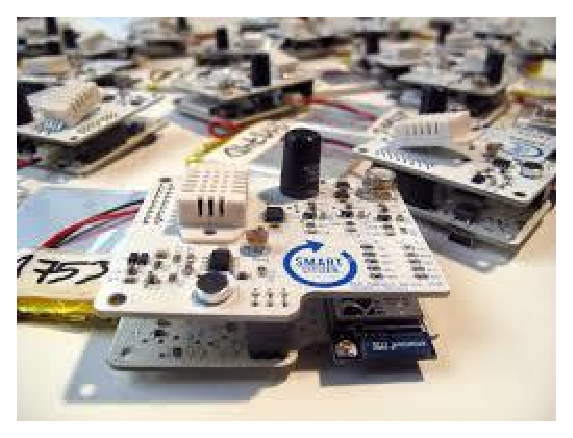
\includegraphics[width=0.40\linewidth]{SCK}
\caption{Smart Citizen Kit units. These are wireless nodes with multiple sensors.}
\label{fig:SCK}
\end{center}
\end{figure}

We are interested in bottom-up models.
We use the terms peer-to-peer, do-it-ourselves and bottom-up interchangeably.
The idea that we want to transmit with bottom-up is that the participant takes an active role and contributes to the community rather than being a mere consumer.
For this reason, we teach the first simple steps to build, configure and program a sensor that uploads the gathered data to the Internet to make it publicly available.

This course is not only listening and reading. 
It is not a course about memorizing data and algorithms and passing tests.
It is a course about programming, prototyping, constructing electronic devices, distributing the data and, in summary, completing projects.
We want the participants to acquire the true and profound understanding necessary to transform their ideas and creativity into reality.
Our goal is to offer true, long-lasting, enjoyable learning.

Our intention is to create a course different from those that already exist.
It is not difficult to find introductory courses to chemistry, physics, biology, economics, etc.
The course that we propose complements the extensive offer of courses which is already available.

Taking this course requires commitment, as the price of the necessary electronic components to work on the assignments is around 100 Euro.
Therefore, our goal regarding the number of participants cannot be quantity.
It has to be quality.

\begin{itemize}
\item We aim at a high completion rate,  our goal is that 100\%  of participants complete a project.
\item We aim at a high collaboration rate, above 80\%.
\item We expect the participants to behave as peers and contribute to improve the course.
We aim at a high contribution rate, above 10\% of the participants should work on making the course better.
\item We aim at creating a community beyond the course.
At least one in-person workshop should be organized to give an opportunity to build and strengthen a community.
\end{itemize}

This course is based on a regular course taught at Universitat Pompeu Fabra.
The lab assignment guide is available in \texttt{github} and \texttt{scribd}: \url{http://www.scribd.com/doc/156136472/A-course-on-Wireless-Sensor-Networks-WSNs}

%------------------------------------------------

\subsection{Methodology}

The course is organized in different units.
Each of the units is a basic ingredient in the construction of a bottom-up wireless sensor network.
For each of the units, we will follow the same class dynamics.

\subsubsection{Class dynamics}

The course is divided in video lectures and written material, both published as the course goes on. Video content includes: teaching lessons, interviews and additional instructions for the assignments (when necessary). While the written material is composed by assignments and self-assessment quizzes. 

Each unit starts with a motivational video introduction delivered by an invited expert introducing fundamental concepts.
Then, a lecturer presents the different concepts, tools and examples that are going to be useful for both the assignments and the self-assessment quizzes.
Starting from the necessary theory underlying each unit, the lecturer then guides the students through hands-on examples providing further insight on the subject.

After each unit's video lessons, assignments are ``unlocked'' to the student. Assignments are composed of written (and photographic) material detailing instructions on how to build examples, which work as hints to complete the assignment itself.

%After completing the assignments, students are provided with all that is required to successfully complete the end-of-unit self-assessment quizzes. These in turn are composed of both theory and assignment-related multiple-choice questions.

Teachers will propose challenges on each assignment, often composed of alternative or advanced services that can be added at various stages with some additional work. Challenges are the ground for a final course project which students may submit and present in a final event.

Challenges may be completed by forming groups of one or more students, in fact, collaboration among groups is encouraged. It is strongly believed that discussion and feedback provide more valuable results and are considered as ways of effective learning in this platform.

Each group of students will own a blog in which the completed assignments will be posted.
The blog should contain links to the code, schematics, demonstration videos and any other material that helps to better understand the work.
For the final project, the groups will also prepare a presentation that will also be included in the blog.

\subsubsection{Badges as a merit recognition system}

This course has the following learning goals:
\begin{itemize}
\item Combine electronics and code in Arduino for sensory and actuation projects.
\item Configure XBees and effectively use them in a communications project.
\item Combining sensors (and probably actuators) with wireless communications and networking to turn creative ideas into working prototypes.
\end{itemize}

By completing assignments, the participants will show their mastery of each of these aspects and will earn a badge as a reward.
Deciding which badges will be offered in the course, the exact criteria to award a badge and designing such badges is one of the tasks of the preparation of the course.


The P2P University offers all the necessary tools to create and award badges.
An example of a badge is shown in Figure~\ref{fig:badge}.

%The participants will watch a motivation video and a video tutorial.
%The tutorial will describe how to complete a simple project and will be complemented.
%Then, the participants have to collaborate to solve a challenge.
%The teachers offer a suggested challenge, but the participants are free to take other challenges that are relevant to them and to the course.
%Finally, the participants have to carefully document their works so that it can be evaluated, reproduced and discussed by the other participants.

%The first and the last unit are slightly different.
%In the first unit there is no project as the focus is on the presentation of the participants, the course itself and the discussion of the expectations on the course.
%The last unit is also special because the participants design, plan, execute and document their own project. 
%The courses finishes with an exhibition of the personal projects.

\begin{figure}
\begin{center}
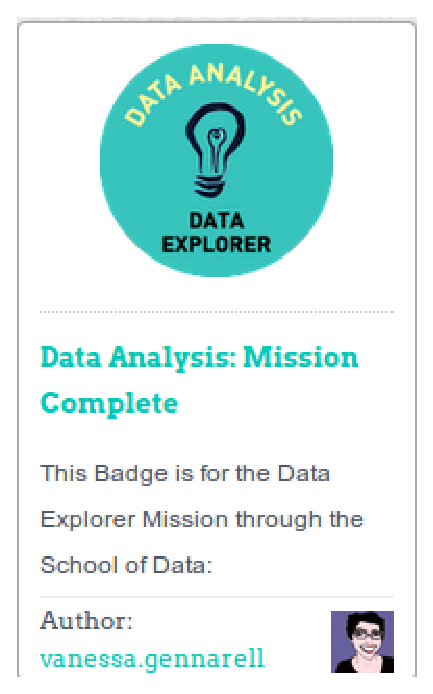
\includegraphics[width=0.40\linewidth]{badge}
\caption{Example of a badge offered at the P2P University}
\label{fig:badge}
\end{center}
\end{figure}
\subsubsection{In-person courses}

Besides the online offer, the course will also be offered in-class for students registered at Universitat Pompeu Fabra.
Furthermore, it will be possible to use the material for Summer Schools to promote the University and Bottom-up Initiatives.

\subsubsection{On-line platform}

As the goal is to reach everyone that has an interest on the construction of wireless sensor networks, the course will also be offered in the P2P University course platform.
This platform will be used to host the videos, written material and tools for discussion and feedback.

In his keynote talk in Edulearn'13 in Barcelona, P2PU co-founder Philipp Schmidt explained that when they conceived P2PU they were looking for something different than Coursera or EdX.
The interest was in building something inexpensive, in a bottom-up fashion, using the resources already available on the web.

The peer-to-peer principles are summarized by the words ``Learning from the people, by the people. About almost anything''.

The P2P is built on strong principles. 
Their web highlights ``open'', ``community'' and ``peer learning''.
Technologies and processes are open to make it open to collaborate.
The organization is horizontal and driven by community discussions.
And everyone is invited to learn and teach using the platform.

The courses are not constricted to the tools of the platform itself. 
On the contrary, they make use of all the resources available in the web such as mailing lists, blogging, micro-blogging, instant messaging, forums and video-conferences. 

\subsubsection{Completion rate, statistics and scientific analysis of the experience}

One of the weaknesses of MOOCs are the low completion rates, typically below 10\%.
The reason is that people registers for courses but do not have the necessary time and/or motivation to complete them.

The goal of the P2PU and the ``mechanicalmooc'' engine is to offer an engaging and enriching experience to the participants, so that everyone benefits from the course.
Preetha Ram, which is involved in the ``mechanicalmooc'' has been quoted to say: ``We want to do more than sign up tens of thousands of students and have only a fraction succeed. Our goal is to have everyone who participates succeed''.

The system includes a logging and analytics system to keep tracks of clicks, emails and engagement in general.
All this data is available for researchers and a team led by June Ahn (University of Maryland) is studying the data to find the best ways to encourage the participation of all registered users \cite{ahn2013dop}

See \url{http://http://info.p2pu.org/research/} for further details.

\subsubsection{In-person Workshops and Meetings}

The participants in nearby locations will be encouraged to meet and gather to work together in the projects.
In-person collaboration provides a far richer experience than on-line work and helps keep people participative and engaged.
Those that cannot meet in person will also be encouraged to get acquainted with their groups with presentation videos and/or other tools for team building.

\subsubsection{Additional Material}

\begin{itemize}
\item Robert Faludi ``Building Wireless Sensor Networks'' \cite{faludi2010bws}
\item Alejandro Andreu ``Open Sensor Network'' \cite{andreu2013osn}
\item Massimo Banzi ``Getting Started with Arduino'' \cite{banzi2009gsa}
\end{itemize}


%------------------------------------------------

\subsection{Work Plan}

\begin{enumerate}
    \item Identifying and specifying the course goals, the assignments and projects to learn and achieve such goals, as well as the evaluation criteria. October 2013. Leader: Jaume Barcelo.
    \item Scripting of the course: preparation of the course structure including units segmentation, number/length of videos per unit, assignments and quiz dynamics and evaluation, feedback and collaboration management; and final project evaluation. November 2013. Leader: Jaume Barcelo.
    \item Preparation of the written guide: there is already a guide for the in-class course, therefore this new adapted guide should take advantage of on-line resources (video, comments, etc.). December 2013. Leader: Luis Sanabria-Russo.
    \item Preparation of the quizzes. 
    Embedded googleforms will be used for the quizzes. January 2014. Leader: Luis Sanabria-Russo.
    \item Preparation of the badges using the P2P University tools. February 2014. Leader: Luis Sanabria-Russo.
    \item Setting up the P2P University on-line platform: based on the course script, this task will configure the platform accordingly. February 2014. Leader: Luis Sanabria-Russo.
    \item Shooting and producing the videos: this final task aims at shooting the videos according to what was designed in the course script and configured in the P2P University platform. March 2014. Leader: Laia Albo.
\end{enumerate}

The course will start on April.
Fig.~\ref{fig:gantt} presents a Gantt chart representation.

\begin{figure}[ftbp]
\begin{center}

\begin{ganttchart}[y unit title=0.4cm,
y unit chart=0.5cm,
vgrid,hgrid, 
title label anchor/.style={below=-1.6ex},
title left shift=.05,
title right shift=-.05,
title height=1,
bar/.style={fill=gray!50},
incomplete/.style={fill=white},
progress label text={},
bar height=0.7,
group right shift=0,
group top shift=.6,
group height=.3,
group peaks={}{}{.2}]{19}
%labels
\gantttitle{Sept.}{2} 
\gantttitle{Oct.}{2} 
\gantttitle{Nov.}{2} 
\gantttitle{Dec.}{2} 
\gantttitle{Jan.}{2} 
\gantttitle{Feb.}{2} 
\gantttitle{Mar.}{2} 
\gantttitle{April}{2}
\gantttitle{May}{2} \\
%tasks
\ganttbar{Specification}{1}{1} \\
\ganttbar{Scripting}{2}{3} \\
\ganttbar{Written guide}{4}{5} \\
\ganttbar{Quizzes}{6}{7} \\
\ganttbar{Badges}{8}{8} \\
\ganttbar{Platform}{9}{10} \\
\ganttbar{Videos}{11}{13} \\
\ganttbar{Course}{15}{19} \\

%relations 
%\ganttlink{elem0}{elem1} 
%\ganttlink{elem1}{elem2} 
%\ganttlink{elem1}{elem3} 
%\ganttlink{elem1}{elem4} 
%\ganttlink{elem1}{elem5} 
%\ganttlink{elem1}{elem6} 
%\ganttlink{elem2}{elem7} 
\end{ganttchart}
\end{center}
\caption{Gantt Chart}
\label{fig:gantt}
\end{figure}


\begin{figure}
\begin{center}
\includegraphics[width=1.00\linewidth]{screenshot}
\caption{A screenshot of a draft of the course at P2P University}
\label{fig:screenshot}
\end{center}
\end{figure}

% \begin{itemize}
% \item Scripting of the course: Preparation of detailed scripts of the content of the videos, the guide and the requirements for the online platform.
% \item Shooting and producing the videos: The videos will be shot and produced according to the script.
% \item Preparation of the written guide: There is already a guide for the in-class course, but it needs to be adapted to the on-line course.
% \item Setting up the P2P University on-line platform: This task involves the actual creation and configuration of the online course.
% \end{itemize}

%\begin{figure}
%\begin{center}
%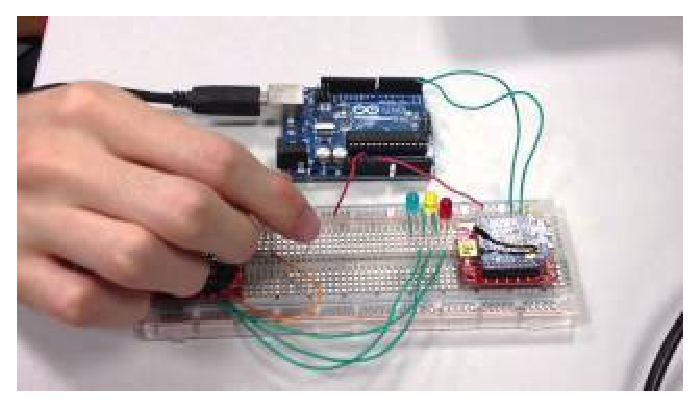
\includegraphics[width=0.40\linewidth]{video}
%\caption{It is necessary to shoot videos with step-by-step instructions to build the projects or complete the assignments.}
%\label{fig:video}
%\end{center}
%\end{figure}
%\begin{figure}
%\begin{center}
%\includegraphics[width=0.40\linewidth]{lesson}
%\caption{Some video lessons will show the teacher's face over supporting slides.}
%\label{fig:lesson}
%\end{center}
%\end{figure}

\subsubsection{Coordination tools}
The tools will be the typical for collaborative projects:
A mailing list for day-to-day progress and weekly meetings.
Also IRC discussions as needed.
Agile methodologies, \emph{Trello} and \emph{Wiggio} will also be considered for project and group management.

%------------------------------------------------

\subsection{Results and Impact}

This course builds upon successful experiences. There is already an existing in-person course that received very good feedback from the students.
The laboratory guide of the course is available in \texttt{github} (\url{https://github.com/jbarcelo/WSNs_lecture_notes}) making it easy for everyone to contribute.
We also published the guide in \texttt{scribd} in late July (\url{http://www.scribd.com/doc/156136472/A-course-on-Wireless-Sensor-Networks-WSNs}) and it was read more than 200 times in August.

Also, the idea of bottom-up smart cities implemented by Smart Citizen was applauded in Kickstarter and received over \$60,000 in crowdfunding. 

The hardware used in the course includes the Digi XBee and the Arduino board. 
This tandem was also used in the best-selling book by Rober Faludi ``Building Wireless Sensor Networks''.
Arduino is a first choice platform for those interested in an introduction to electronics and micro-controllers.
More than one million Arduino have been sold, confirming the success of their open business model.

The main goal of this course is to strengthen the community by teaching very basic skills to a large audience. After completing the course, the participants will be able to continue on their own with more advanced projects. 

It is a basic digital education for everyone. People with no or little background in technology will make their first steps into programming, electronics, and sensing projects.

Students successfully completing this course will possess the basic tools to contribute to the creation of bottom-up Smart Cities.

\subsubsection{Results obtained so far}

By simply creating this document and discussing it with the involved communities on the Internet, we have received many inputs, ideas, and encouragement that has helped further shape the idea.

\subsubsection{Eternal work-in-progress}

Many collaborative projects never come to an end.
These projects keep evolving and improving, and the actual direction of the evolution is highly dependant of the people that is working in it in every moment.
The idea is to keep gathering feedback from the participants and use that information to continuously improve the course.
For this reason it is very important that everyone involved does not feel like a simple ``consumer''.
The goal is that the participants are also the ``makers'' of the course and everyone learns from everyone in a peer-to-peer way.


%------------------------------------------------

\subsection{Teaching Plan}

\subsubsection{Concepts and competences acquired in the course}
\begin{itemize}
\item Bottom-up, peer-to-peer and community-oriented collaboration models
\item Sensors, actuators, sensor networks, open data, Smart Cities
\item Basic electronics
\item Basic microprocessor programming
\item Configuration of Digi XBee
\item ZigBee communication
\end{itemize}


\subsubsection{Weekly organization}
\begin{itemize}
\item Week 1: Presentation of the participants, presentation of the course, motivation to take the course, dream about a personal project.
\item Week 2: Introduction to Arduino. Arduino IDE. Input/output. \\\underline{Lab assignment}: Blinking LED project.
\item Week 3: Introduction to XBee. Basic configuration of AT mode. \\\underline{Lab assignment}: ZigBee chat project.
\item Week 4: Basic interaction. Make a measurement and react. \\\underline{Lab assignment}: Wireless Sunset Sensor project.
\item Week 5: Open data. The importance of sharing the data. Open data platforms. \\\underline{Lab assignment}: Taking measures with a sensor and uploading them to the Internet.
\end{itemize}

Motivating videos:
\begin{itemize}
\item Do-it-ourselves, Bottom-up, Sensors, Smart Cities, Smart Cities Kit:
Laia Albo, Michel Bauwens, Tiberius Brastaviceanu, Guillem Camprodon and Tomas Diez, Alex Posada

\item Arduino (Blinking LED):
David Mellis, (Jaume Barcelo)

\item XBee (Chat):
Robert Faludi, (Luis Sanabria-Russo)

\item Interaction design (Sunset Sensor):
Alex Posada (Luis Sanabria-Russo)

\item Open Data, Open Data platforms (Internet thermometer):
Albert Domingo, Manuel Palacin, (Alejandro Andreu)
\end{itemize}


%------------------------------------------------

\subsection{Lead teacher}
\begin{itemize}
\item Jaume Barcelo (Universitat Pompeu Fabra): He is a lecturer at Universitat Pompeu Fabra where he takes part in the Wireless Sensor Network course. He has also taught at Universidad Carlos III de Madrid where he collaborated with the opencourseware experience that published the class materials online. Together with Luis Sanabria, he has prepared the basic laboratory guide for the Wireless Sensor Networks course that has been shared with the Internet community. Jaume has taught more than 20 courses at the graduate and undergraduate level at two universities. Visit www.jaumebarcelo.info for more information.
\begin{center}

\includegraphics[width=0.200\linewidth]{jaume}
\label{fig:jaume}
\end{center}
\end{itemize}


\subsection{Other members of the team}
\begin{itemize}
\item Laia Albo (Universitat Pompeu Fabra): She is a research technician at Telefonica-UPF chair ``Social Innovation in Education''. Audiovisual Systems Engineer from the University Pompeu Fabra, she has worked in the Teaching Quality and Innovation Support Unit (USQUID) of the Polytechnic School of the UPF to support the project linked to the creation of educational videos for academic support (both for teachers and students).
\begin{center}
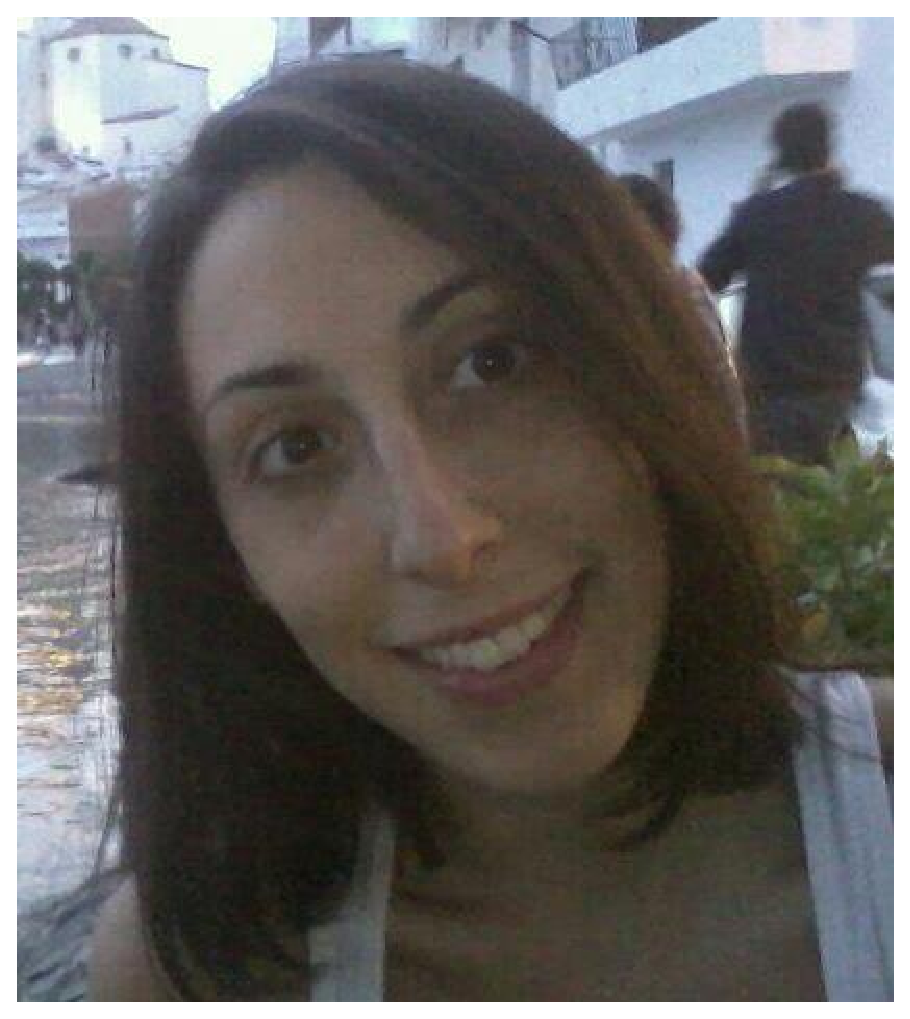
\includegraphics[width=0.200\linewidth]{laia}
\label{fig:jaume}
\end{center}
\item Alejandro Andreu (Universitat Pompeu Fabra): He completed his degree on Computer Communications with a thesis entitled ``Open Sensor Networks''. He has also contributed to the Smart Citizen Kit project.
\begin{center}

\includegraphics[width=0.200\linewidth]{alejandro}
\label{fig:jaume}
\end{center}
\item David Mellis (Arduino)
\item Michel Bauwens (P2P Foundation)
\item Tiberius Brastaviceanu (Sensorica): He is founder, active member, coordinator, facilitator, engineer and product designer at Sensorica.
\begin{center}

\includegraphics[width=0.200\linewidth]{tiberius}
\end{center}
\item Guillem Camprodon (FabLab Barcelona): He is a researcher at the Institut d'Arquitectura Avancada de Catalunya (IAAC). He participates in the Smart Citizen Kit project as the main responsible for integration and project development (hardware and software).
\begin{center}
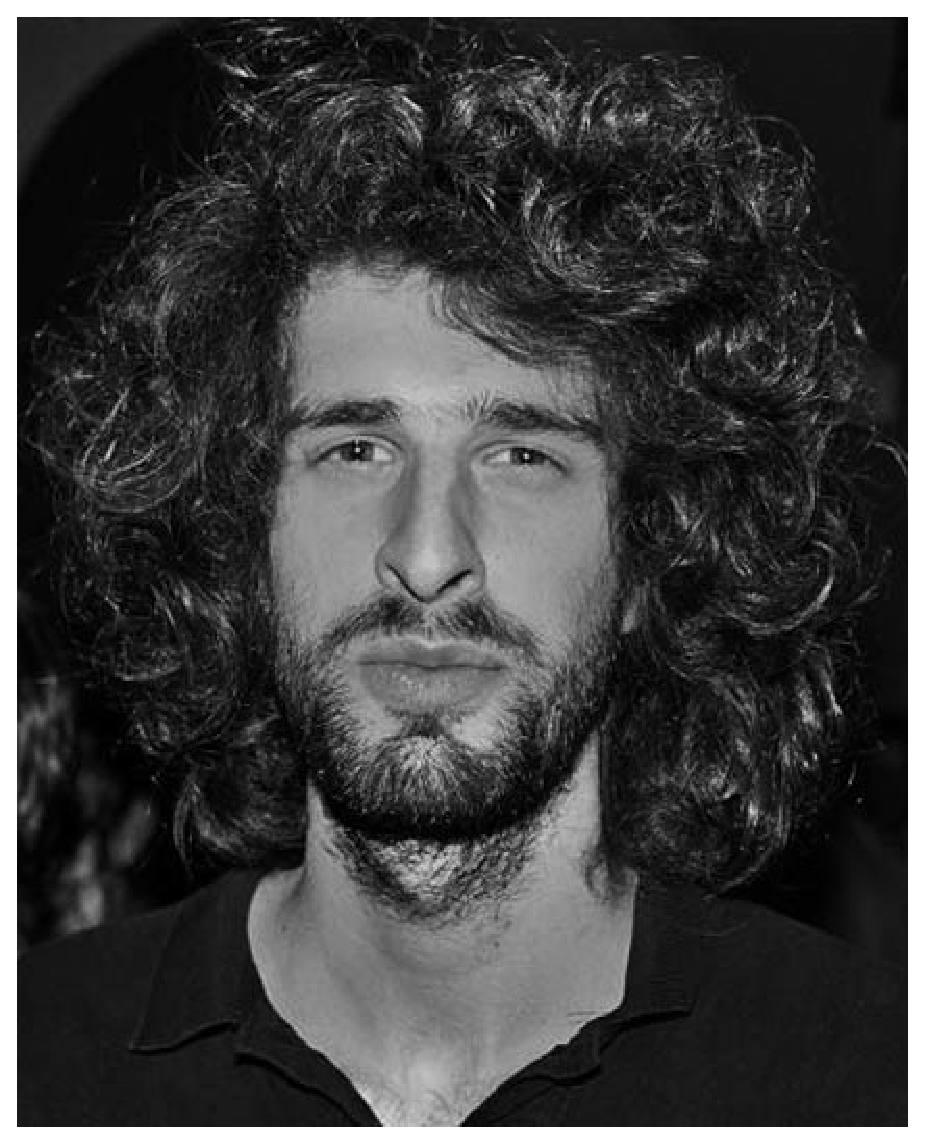
\includegraphics[width=0.200\linewidth]{guillem}
\end{center}
\item Tomas Diez (FabLab Barcelona): He is the director of FabLab Barcelona at the Institut d'Arquitectura Avancada de Catalunya (IAAC) and co-founder of the Smart Citizen Kit initiative. Tomas is also part of the master programs taught at IAAC.
\begin{center}

\includegraphics[width=0.200\linewidth]{tomas}
\end{center}
\item Albert Domingo (Universitat Pompeu Fabra):
He is currently a Ph.D. candidate at the Networking Technologies and Strategies (NeTS) group at UPF. He has also been a visitor with the Advanced Network Architecture group at MIT.

He is a teaching assistant in a course about networking protocols. His research interests include Super-Wifi communications, Open Data, Big Data, public administration data and regulation. He participates in the 'Commons for Europe' and 'Open Cities' European projects. 
\begin{center}
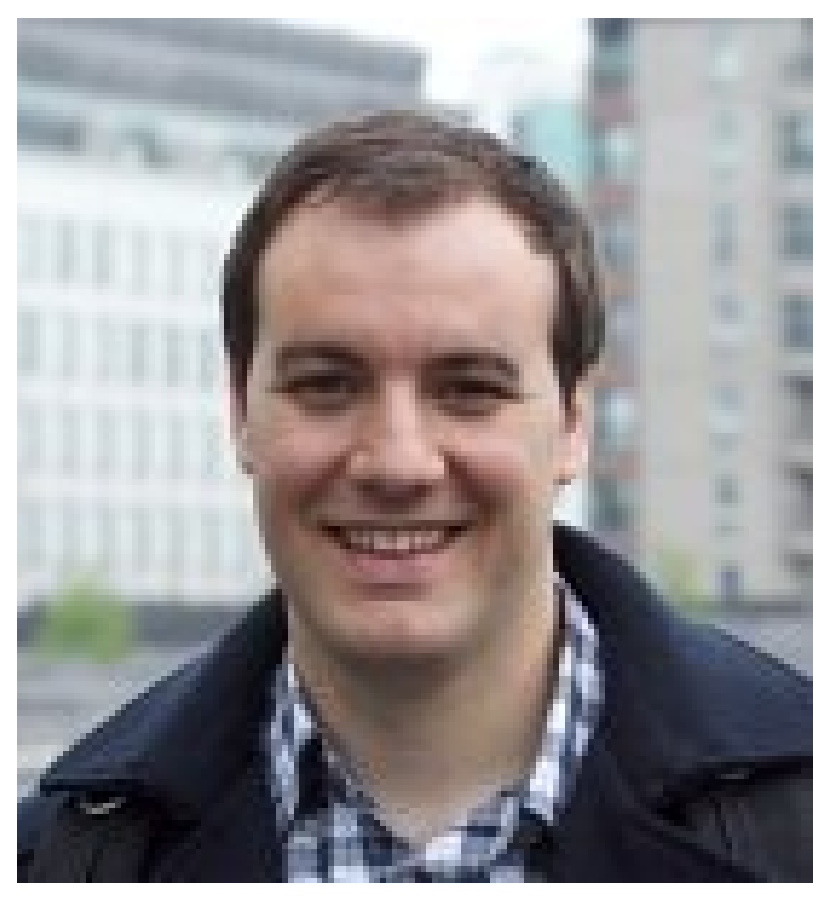
\includegraphics[width=0.200\linewidth]{albert}
\end{center}
\item Robert Faludi (Digi International)
\item Vanessa Gennarelli (P2P University): She is Learning Lead at P2PU.
\begin{center}
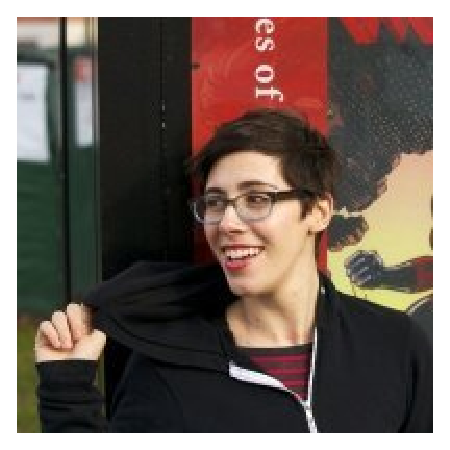
\includegraphics[width=0.200\linewidth]{vanessa}
\end{center}
\item Luis Sanabria-Russo (Universitat Pompeu Fabra): He is a Ph.D. student in the Department of Information and Communication Technologies. He has taught a course in Wireless Sensor Networks and has been involved in the preparation of audiovisual material for online courses.

\begin{center}
\includegraphics[width=0.200\linewidth]{luis}
\label{fig:luis}
\end{center}
\item Manuel Palacin (Universitat Pompeu Fabra): Manuel is a Ph.D. candidate working on open data platforms.
\item Alex Posada (Media Interaction Design Lab): He is the founder and CEO at Media Interactive Design (MID) and also coordinates the Interaction Lab at hangar.org . Alex teaches in the Master of Advanced Architecture and the Master of Advanced Interaction at the Institut d'Arquitectura Avancada de Catalunya (IAAC). Alex is a co-founder of the Smart Citizen Kit initiative. He is also the director of the interaction lab at Hangar Barcelona (www.hangar.org).
\begin{center}

\includegraphics[width=0.200\linewidth]{alex}
\end{center}
\item And you, if you want. Everyone is invited to join the team and collaborate.
\end{itemize}



\section{Conclusion}
\label{sec:conclusion}
This report covers the training and networking efforts in the BuB4EU branch of the Commons for Europe project.
As fellows are actively participating in this project, it is of paramount importance to provide them with help and guidance to make sure that they can accomplish their goals.
Each student is assigned both an experienced BuB mentor and an academic advisor, which have complementing roles.

As we are interested in bottom up initiatives, it is very important to build a community with people and links that span beyond the consortium.
To this end, we maintain an open mailing list and organize open workshops to attract new participants interested in the BuB concept.



% if have a single appendix:
%\appendix[Proof of the Zonklar Equations]
% or
%\appendix  % for no appendix heading
% do not use \section anymore after \appendix, only \section*
% is possibly needed

% use appendices with more than one appendix
% then use \section to start each appendix
% you must declare a \section before using any
% \subsection or using \label (\appendices by itself
% starts a section numbered zero.)
%


%\appendices
%\section{Proof of the First Zonklar Equation}
%Appendix one text goes here.

% you can choose not to have a title for an appendix
% if you want by leaving the argument blank
%\section{}
%Appendix two text goes here.


% use section* for acknowledgement
\section*{Acknowledgment}

This work has been partially funded by the European Commission (grant CIP-ICT PSP-2011-5).
The views expressed in this technical report are solely those of the authors and do not represent the views of the European Commission.


% Can use something like this to put references on a page
% by themselves when using endfloat and the captionsoff option.
%\ifCLASSOPTIONcaptionsoff
%  \newpage
%\fi



% trigger a \newpage just before the given reference
% number - used to balance the columns on the last page
% adjust value as needed - may need to be readjusted if
% the document is modified later
%\IEEEtriggeratref{8}
% The "triggered" command can be changed if desired:
%\IEEEtriggercmd{\enlargethispage{-5in}}

% references section

% can use a bibliography generated by BibTeX as a .bbl file
% BibTeX documentation can be easily obtained at:
% http://www.ctan.org/tex-archive/biblio/bibtex/contrib/doc/
% The IEEEtran BibTeX style support page is at:
% http://www.michaelshell.org/tex/ieeetran/bibtex/
\bibliographystyle{IEEEtran}
% argument is your BibTeX string definitions and bibliography database(s)
\bibliography{IEEEabrv,my_bib}
%
% <OR> manually copy in the resultant .bbl file
% set second argument of \begin to the number of references
% (used to reserve space for the reference number labels box)
%\begin{thebibliography}{1}

%\bibitem{IEEEhowto:kopka}
%H.~Kopka and P.~W. Daly, \emph{A Guide to \LaTeX}, 3rd~ed.\hskip 1em plus
%  0.5em minus 0.4em\relax Harlow, England: Addison-Wesley, 1999.

%\end{thebibliography}

% biography section
% 
% If you have an EPS/PDF photo (graphicx package needed) extra braces are
% needed around the contents of the optional argument to biography to prevent
% the LaTeX parser from getting confused when it sees the complicated
% \includegraphics command within an optional argument. (You could create
% your own custom macro containing the \includegraphics command to make things
% simpler here.)
%\begin{biography}[{\includegraphics[width=1in,height=1.25in,clip,keepaspectratio]{mshell}}]{Michael Shell}
% or if you just want to reserve a space for a photo:

%\begin{IEEEbiography}{Michael Shell}
%Biography text here.
%\end{IEEEbiography}

% if you will not have a photo at all:
%\begin{IEEEbiographynophoto}{John Doe}
%Biography text here.
%\end{IEEEbiographynophoto}

% insert where needed to balance the two columns on the last page with
% biographies
%\newpage

%\begin{IEEEbiographynophoto}{Jane Doe}
%Biography text here.
%\end{IEEEbiographynophoto}

% You can push biographies down or up by placing
% a \vfill before or after them. The appropriate
% use of \vfill depends on what kind of text is
% on the last page and whether or not the columns
% are being equalized.

%\vfill

% Can be used to pull up biographies so that the bottom of the last one
% is flush with the other column.
%\enlargethispage{-5in}



% that's all folks
\end{document}


